% first i tried to use org mode, but that doesn't have sufficient
% support for formulas and images
\documentclass[11pt]{article}
\usepackage[utf8]{inputenc}
\usepackage[T1]{fontenc}
\usepackage{graphicx}
\usepackage{longtable}
\usepackage{float}
\usepackage{wrapfig}
\usepackage{soul}
\usepackage{amssymb}
\usepackage{hyperref}
\usepackage{color}

\title{aberration}
\author{martin}
\date{31 March 2011}

\begin{document}

\maketitle

\setcounter{tocdepth}{3}
\tableofcontents
\vspace*{1cm}
\section{Aberration due to water}
\label{sec-1}

\subsection{Refraction on thin lens}
\label{sec-1.1}
\subsection{Refraction through oil objective}
\label{sec-1.2}

\subsection{Refraction at plane surface}
\label{sec-1.3}

   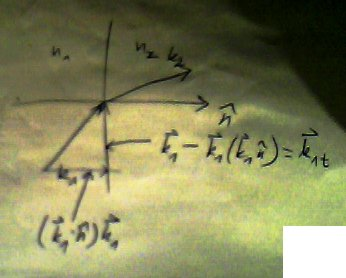
\includegraphics[width=10em]{./slab.jpg}

   
\subsubsection{Result in terms of wavevector}
\label{sec-1.3.1}

 

\subsubsection{}
cg-principles.djvu foley addison-wesley 1990
 \begin{figure} 
   \centering
   %\def\svgwidth{\columnwidth} % sets the image width, this is optional
   \input{refl2.pdf_tex}
 \end{figure}

\end{document}
